% =====================================================================
%  Does the timescape cosmology resolve the Hubble tension?
%  Dressed-Hubble consistency and the covariance-sensitivity of the
%  Pantheon+ supernova evidence.
%
%  DRAFT for arXiv (astro-ph.CO / gr-qc). Compile: pdflatex x2.
%  Class: revtex4-2.  Figures fig_dbic.pdf, fig_hubble.pdf in same dir.
%
%  >>> BEFORE SUBMITTING <<<
%   (1) Fill in affiliation (currently "Independent Researcher").
%   (2) arXiv ids machine-verified vs live arXiv 2026-06-06 (all 12 resolve); fixed CCHP2025 first author (Hoyt) + Wiltshire2014 publisher; confirm Phys.~Rept. vol/page before final submission.
%   (3) astro-ph.CO/gr-qc need an endorsement for a first-time submitter.
% =====================================================================
\documentclass[aps,prd,twocolumn,nofootinbib,superscriptaddress,floatfix]{revtex4-2}
\usepackage{amsmath,amssymb}
\usepackage{graphicx}
\usepackage{booktabs}
\usepackage{hyperref}
\hypersetup{colorlinks=true,linkcolor=blue,citecolor=blue,urlcolor=blue}

\newcommand{\Ho}{H_{0}}
\newcommand{\Hbaro}{\bar H_{0}}
\newcommand{\fvo}{f_{v0}}
\newcommand{\kmsmpc}{\,\mathrm{km\,s^{-1}\,Mpc^{-1}}}
\newcommand{\Lcdm}{\Lambda\mathrm{CDM}}
\newcommand{\dBIC}{\Delta\mathrm{BIC}}

\begin{document}

\title{Can eliminating dark energy resolve the Hubble tension?
A uniform test of void and backreaction cosmologies against
supernovae, baryon acoustic oscillations, and the CMB acoustic scale}

\author{Viacheslav Zhygulin}
\email{s.zhygulin@gmail.com}
\affiliation{Independent Researcher}
\date{\today}

\begin{abstract}
\footnotesize
The timescape cosmology of Wiltshire dispenses with dark energy, attributing
apparent acceleration to the backreaction of inhomogeneities and the associated
wall--void clock-rate difference, and has been claimed to ease the Hubble
tension. We test two distinct claims. First, treating the published timescape
determinations of the dressed Hubble constant as fixed, we show with an explicit
tension statistic that the early-Universe (CMB, $61.0\kmsmpc$) and late-Universe
(supernova, $61.7\kmsmpc$) values are mutually consistent to $\lesssim0.5\sigma$,
against $\approx4.9\sigma$ for the $\Lcdm$ interpretation of the same data, and
that the fractional excess required to reconcile the local distance-ladder value
($+18.4\%\pm2.8\%$) lies within the independently-predicted $17$--$22\%$
void-scale expansion variance. Because the global dressed value
($\approx\!61$) sits below \emph{both} canonical numbers, this is a recasting of
the tension as a scale-dependent measurement artifact, not a reconciliation near
$70\kmsmpc$. This agreement is calibration-relative: a fresh
SH0ES-calibrator-anchored fit within our own machinery gives a late-time dressed
$\Ho=73.0\pm1.0\kmsmpc$---the locally-biased value timescape itself predicts
(required fractional excess $0.197$, within the same $17$--$22\%$ window)---so
claim~(A) rests on the expansion-variance recasting, not on an $\Ho$ coincidence
at $61$. Second, we independently reanalyse Pantheon$+$, implementing the
timescape distance--redshift relation from first principles and validating the
pipeline three ways. We find the model comparison is strongly sensitive to the
covariance treatment: with the full statistical$+$systematic covariance, flat
$\Lcdm$ is favoured under every magnitude standardisation we test
($\dBIC=+3.9$ to $+5.1$, and $+9.0$ with the bias correction removed), and the
timescape void fraction rails to $\fvo\approx0.85$; a timescape preference
($\dBIC\approx-8$) emerges only when the off-diagonal covariance is
\emph{discarded}. Exact Bayes factors track this: the full covariance gives
$\ln B=+1.3$ to $+1.8$ for $\Lcdm$, while the cosmology-independent stat-only
reduction gives $\ln B=5.4$--$5.9$ for timescape, reproducing the proponents'
$\ln B>5$ purely from the covariance treatment. Running the comparison directly
under the now-public cosmology-independent covariance of Seifert et al.\ (2025),
our frequentist fit reproduces the published maximum-likelihood value
($\fvo=0.675$, $\Omega_{m0}=0.433$) \cite{Lane2025} and recovers the reported
redshift-cut dependence: timescape is marginally favoured below the
statistical-homogeneity scale ($\dBIC=-0.5$ at $z>0.01$) and $\Lcdm$ above it
($\dBIC=+4.9$ at $z\geq0.055$). The supernova preference is therefore real but
scale-dependent---a low-redshift effect rather than a robust whole-sample
preference---which sharpens rather than overturns our localisation of it to the
low-$z$ regime. Third, we calibrate timescape against DESI DR2
baryon-acoustic-oscillation (BAO) distances and the Planck acoustic scale: this
recovers the published timescape CMB void fraction ($\fvo\simeq0.64$, dressed
$\Ho\simeq63\kmsmpc$) but fits worse than $\Lcdm$
($\chi^2/\mathrm{dof}=6.7$ vs $0.89$) and prefers a void fraction in tension with
the supernova-preferred value ($\fvo\simeq0.64$ vs $0.74$--$0.85$). The
supernova-versus-BAO void-fraction split is a $4.8\sigma$ profile-likelihood
parameter-shift in the CMB- and $r_d$-independent BAO-only pairing ($6.6\sigma$
including the CMB point, with a $3.1\sigma$ floor across supernova reductions),
softening to $\sim1$--$2\sigma$ only under the external cosmology-independent
anchor combined with the CMB $\fvo$ systematic grafted onto the geometric fit; a
parametric bootstrap excludes a single void fraction at $\gtrsim3.2\sigma$. We
therefore report a robust shape tension, to be settled definitively only with a
self-consistent timescape sound horizon---within timescape the early/late $\Ho$
numbers themselves reconcile at $\approx61\kmsmpc$. Applying the identical test to
the wider void/backreaction family (LTB, R\"as\"anen, Buchert morphon, Szekeres,
KBC local void) yields the same SN--BAO$+$CMB parameter split in every
dark-energy-free model and none reaching the local $\Ho$, the LTB subclass being
independently excluded by the kinetic Sunyaev--Zel'dovich effect. We note that
the tension's size is calibrator-dependent: the tip-of-the-red-giant-branch ladder
(CCHP) gives $\Ho\simeq68$--$70$, only $\sim1$--$1.5\sigma$ from Planck, so the
$5\sigma$ tension is largely specific to the SH0ES Cepheid calibration. On present
public data, eliminating dark energy via inhomogeneity does not resolve the
Hubble tension.
\end{abstract}

\maketitle

\section{Introduction}
\label{sec:intro}

The Hubble tension is the disagreement between late- and early-Universe
determinations of $\Ho$. The local Cepheid$+$type~Ia supernova (SN~Ia)
measurement of SH0ES is $\Ho=73.04\pm1.04\kmsmpc$ \cite{Riess2022}; the Planck
CMB value under spatially-flat $\Lcdm$ is $\Ho=67.36\pm0.54\kmsmpc$
\cite{Planck2018}; the discrepancy is quoted at $5\sigma$. JWST rules out
Cepheid crowding as the cause at $8.2\sigma$ \cite{Riess2024JWST}. The picture is,
however, calibrator-dependent: the tip-of-the-red-giant-branch (TRGB) ladder of
the Chicago--Carnegie Hubble Program gives a markedly lower
$\Ho\simeq68$--$70\kmsmpc$ \cite{Freedman2024,CCHP2025}---only $\sim\!1$--$1.5
\sigma$ above Planck---and baryon-acoustic inverse-distance-ladder values remain
near $68$ \cite{DESI2024}. The strong $5\sigma$ tension is therefore largely
specific to the SH0ES Cepheid calibration; the target a late-Universe model must
reach is $\sim\!69$ if one adopts the TRGB ladder, or $73$ for Cepheids.

A logically distinct class of resolution questions the homogeneous
Friedmann--Lema\^itre--Robertson--Walker (FLRW) interpretation itself. The
timescape cosmology of Wiltshire \cite{Wiltshire2007,Wiltshire2009} models the
present, void-dominated Universe as a two-phase Buchert average
\cite{Buchert2000}: spatially-flat ``walls'' (bound structures, where observers
sit) and negatively-curved ``voids.'' A quasilocal gravitational-energy and
clock-rate gradient means a wall observer fitting FLRW infers ``dressed''
parameters distinct from the volume-average ``bare'' ones; apparent acceleration
follows without dark energy. Recent Bayesian comparisons against Pantheon$+$
report strong evidence for timescape over $\Lcdm$ \cite{Seifert2024,Lane2025},
reviving the question of whether the framework also addresses the Hubble tension.

The popular framing conflates two claims that are not equivalent: \textbf{(A)}
within timescape the early- and late-Universe dressed Hubble constants
\emph{agree}; and \textbf{(B)} timescape \emph{resolves} the $67$-versus-$73$
tension. We show (Sec.~\ref{sec:consistency}) that (A) holds at high precision
while (B) holds only in a specific sense. We then ask whether the supernova
evidence is robust (Sec.~\ref{sec:sne}); we find the preference is contingent on
the covariance treatment.

\paragraph*{Originality.} The framework relations of Sec.~\ref{sec:framework}
and the published best-fit parameters are due to Wiltshire and collaborators and
are reproduced for self-containment. New here are: the explicit tension statistic
and local-excess cross-check of Sec.~\ref{sec:consistency}; and the independent
Pantheon$+$ reanalysis of Sec.~\ref{sec:sne}, in particular the localisation of
the timescape preference to the discarding of the off-diagonal covariance. All
code is available (Sec.~\ref{sec:avail}). This is a timescape-specific study; it
does not survey other void/inhomogeneous models (LTB, Szekeres, general Buchert
closures), which the same pipeline could test in future work.

\section{Timescape framework}
\label{sec:framework}

We use only what is needed; see \cite{Wiltshire2007,Wiltshire2009} for
derivations. The void volume fraction $f_v(t)$ grows to a present value $\fvo$.
The lapse $\bar\gamma\equiv dt/d\tau_w$ relates volume-average time $t$ to wall
proper time $\tau_w$, and in the late-time tracker solution the dressed and bare
Hubble parameters are related by \cite[eq.~(B9)]{Wiltshire2009}
\begin{equation}
\Ho=\frac{4\fvo^{2}+\fvo+4}{2(2+\fvo)}\,\Hbaro,\qquad
\bar\gamma_0=\tfrac12(2+\fvo).
\label{eq:dressed}
\end{equation}
The bare deceleration parameter stays positive while the dressed one turns
negative for $f_v\gtrsim0.59$. Best fits give dressed $\Ho\approx61.7$ and bare
$\Hbaro\approx50\kmsmpc$ \cite{Leith2008,Duley2013}.

\section{Dressed-Hubble consistency and resolution-vs-recasting}
\label{sec:consistency}

We quantify agreement by $T_{AB}=|\Ho^A-\Ho^B|/\sqrt{\sigma_A^2+\sigma_B^2}$.

\emph{$\Lcdm$ reference.} For SH0ES versus Planck,
$T=5.68/\sqrt{1.04^2+0.54^2}=4.85$ ($\approx5\sigma$ as quoted) \cite{Riess2022}.

\emph{Timescape.} The CMB-calibrated dressed value is $61.0\kmsmpc$
($\pm0.79$ stat, $\pm4.88$ sys) \cite{Nazer2015} and the SN-calibrated value is
$61.7^{+1.2}_{-1.1}\kmsmpc$ \cite{Leith2008,Wiltshire2009}; the residual is
$0.7\kmsmpc$, so $T^{\rm TS}=0.50$ (stat) or $0.14$ (stat$\oplus$sys). The same
statistic that registers $4.85\sigma$ for the $\Lcdm$ reading registers
$\lesssim0.5\sigma$ for the timescape reading, establishing claim~(A).

\emph{Local-excess cross-check.} Timescape predicts that a wall observer infers
an apparent $\Ho$ biased high below the $\sim\!100\,h^{-1}$Mpc homogeneity scale,
peaking near the $\sim\!30\,h^{-1}$Mpc dominant-void scale
\cite{Wiltshire2009,Smale2011}. The excess required to reconcile SH0ES with the
dressed asymptote, $\delta_{\rm req}=73.04/61.7-1=0.184\pm0.028$, lies within the
predicted $\sim\!17$--$22\%$ apparent-Hubble variance (local maxima
$\sim\!75\kmsmpc$) \cite{Wiltshire2009}. This is a magnitude-consistency
argument: the SH0ES Hubble-flow sample extends to $z\sim0.15$, beyond the
homogeneity scale, so the account relies additionally on the cosmic-rest-frame
choice, for which \cite{Wiltshire2013} report evidence favouring the Local Group
frame.

\emph{Resolution versus recasting.} The global dressed value
($\approx\!61\kmsmpc$) lies below \emph{both} $67.4$ and $73.0$. Timescape does
not split the difference near $70$; it reinterprets both canonical values as
biased relative to a lower global average. This is a \emph{recasting} of the
tension as an FLRW-interpretation artifact, with consequences for consistency
with inverse-distance-ladder BAO \cite{DESI2024} not yet established for
timescape at $\Lcdm$ precision.

\emph{A fresh late-time anchor.} The $\lesssim0.5\sigma$ agreement above pairs the
CMB-calibrated $61.0\kmsmpc$ with the 2008-era SN-calibrated $61.7\kmsmpc$, both
tied to early-Universe or literature calibrations. Executing decisive
test~(ii) of Sec.~\ref{sec:future}---replacing the literature late value with a
fresh SH0ES-calibrator-anchored dressed $\Ho$ measured inside the identical
machinery (validation gate: the flat-$\Lcdm$ anchored fit recovers
$\Ho=73.5\pm1.0\kmsmpc$ and $\Omega_{m0}=0.33$, matching \cite{Brout2022})---yields
a fresh timescape dressed $\Ho=73.0\pm1.0\kmsmpc$ ($\fvo=0.853$, $M_B=-19.24$).
This is expected, not a falsification: anchoring to the local Cepheid ladder pins
$\Ho$ to precisely the value a wall observer is predicted to infer biased high,
and the required fractional excess
$\delta_{\rm req}=\Ho^{\rm local}/\Ho^{\rm dressed}-1=0.197\pm0.023$ lies inside
the predicted $17$--$22\%$ apparent-Hubble-variance window. The $\approx9\sigma$
gap between this local-anchored $73.0$ and the CMB-calibrated dressed asymptote
$61.0$ is thus the model's own predicted local bias, not an anomaly. Claim~(A)
accordingly rests on this expansion-variance argument---a recasting---and never on
an $\Ho$ agreement at $61$; making the late value a fresh measurement makes that
dependence explicit.

\section{Independent reanalysis of Pantheon$+$ supernovae}
\label{sec:sne}

\subsection{Data, models, likelihood}
We use the Pantheon$+$ release \cite{Scolnic2022,Brout2022}; the cosmology
sample is the $N=1580$ SNe with $z_{\rm HD}>0.01$ that are not Cepheid
calibrators ($0.010<z<2.26$). For flat $\Lcdm$,
$d_L=(1+z_{\rm hel})(c/\Ho)\int_0^{z_{\rm HD}}dz'/E(z')$. For timescape we
implement the dressed luminosity distance from \cite[App.~A]{Dam2017} verbatim:
$d_L=(1+z)^2d_A$, $d_A=c\,t^{2/3}[F(t_0)-F(t)]$ with
\begin{align}
F(t)&=2t^{1/3}+\frac{b^{1/3}}{6}\ln\frac{(t^{1/3}+b^{1/3})^2}
     {t^{2/3}-b^{1/3}t^{1/3}+b^{2/3}}\nonumber\\
   &\quad+\frac{b^{1/3}}{\sqrt3}\tan^{-1}\frac{2t^{1/3}-b^{1/3}}{\sqrt3\,b^{1/3}},
\end{align}
$1+z=2^{4/3}t^{1/3}(t+b)/[\fvo^{1/3}\Hbaro\,t(2t+3b)^{4/3}]$,
$b=2(1-\fvo)(2+\fvo)/(9\fvo\Hbaro)$, and (\ref{eq:dressed}). Only $\fvo$ or
$\Omega_{m0}$ shapes the Hubble diagram. We compare by $\dBIC$ (equal nuisance
counts), adopting the Kass--Raftery scale \cite{KassRaftery1995}, marginalising
the absolute-magnitude/$\Ho$ offset analytically.

\subsection{Pipeline validation}
Three independent checks: (i) our flat-$\Lcdm$ fit gives
$\Omega_{m0}=0.333\pm0.018$, matching the published Pantheon$+$ value
\cite{Brout2022}; (ii) $F'(t)$ reproduces the integrand
$2/[(2+f_v)t^{2/3}]$ to machine precision; (iii) our numerical low-$z$ Taylor
coefficient of $\mu_{\rm TS}(z)$ matches the analytic expression of
\cite{Dam2017} to $\sim\!10^{-4}$ across $\fvo\in[0.6,0.8]$.

\subsection{Covariance sensitivity}
We vary two axes: the apparent magnitude---the standard bias-corrected
$m_{B,\rm corr}$ versus a raw SALT2 Tripp combination
$m_B+\alpha x_1-\beta c$ \cite{Tripp1998} with no FLRW-fiducial BBC bias
correction---and the covariance---the full public statistical$+$systematic
matrix $C$ versus its diagonal. Results are in Table~\ref{tab:fits} and
Fig.~\ref{fig:dbic}.

With the \emph{full} covariance, $\Lcdm$ is favoured for \emph{every} magnitude
definition ($\dBIC=+3.9$ to $+5.1$; $+9.0$ if the bias correction is removed),
and the timescape void fraction rails high ($\fvo\approx0.85$--$0.90$, implying a
strongly void-dominated dressed $\Omega_{m0}\approx0.2$). A timescape preference
($\dBIC\approx-8$) appears \emph{only} in the raw-Tripp$+$diagonal corner---i.e.
only when the off-diagonal covariance is discarded. A fully marginalised
statistical-only Tripp fit (fitting $\alpha,\beta,\sigma_{\rm int}$) gives
$\dBIC=-9.4$, consistent with this corner. The driver of any timescape
preference is therefore the suppression of the off-diagonal covariance, not the
magnitude standardisation alone. Figure~\ref{fig:hubble} shows the
near-degeneracy of the two distance--redshift relations ($<0.05$ mag) that makes
the comparison so sensitive.

Exact one-dimensional-quadrature Bayes factors remove any objection that the
$\dBIC$ is a crude approximation. With the full statistical$+$systematic
covariance, $\ln B(\Lcdm/\mathrm{TS})=+1.3$ to $+1.8$ across a $2\times2$ prior
grid (Kass--Raftery ``positive'', favouring $\Lcdm$; smaller than $\dBIC/2$
because $\Lcdm$ carries a $\sim\!1$-nat larger Occam
factor\footnote{The maximised-likelihood ratio favours $\Lcdm$ by
$\Delta\chi^2/2\approx2.6$, but $\Lcdm$'s prior-to-posterior compression costs
$\approx1$ nat more than timescape's, so $\ln B\approx\Delta\chi^2/2-1\approx1.6$.}).
By contrast the cosmology-independent stat-only Tripp reduction gives
$\ln B=5.4$--$5.9$ \emph{for} timescape (``very strong''), reproducing in-house the
$\ln B>5$ of \cite{Seifert2024} purely from the covariance treatment: the sign of
the evidence is set by whether the off-diagonal terms are retained or rebuilt, not
by the model. A parametric bootstrap calibrates the frequentist significance:
were timescape true, the observed supernova-only $\dBIC=+5.1$ in $\Lcdm$'s favour
would arise with probability $p=0.008$ ($2.4\sigma$; 4000 mocks drawn from the
full stat$+$sys covariance).

\begin{table}[t]
\caption{Timescape vs flat $\Lcdm$ on Pantheon$+$: $\dBIC$ (timescape$-\Lcdm$;
$<0$ favours timescape) across magnitude $\times$ covariance. $\Lcdm$ wins under
the full covariance regardless of magnitude; timescape wins only when the
off-diagonal covariance is dropped.}
\label{tab:fits}
\begin{ruledtabular}
\begin{tabular}{lcc}
Magnitude & Full cov & Diagonal\\
\colrule
$m_{B,\rm corr}$ (standard, bias-corr.)   & $+5.1$ & $+4.9$\\
$m_{B,\rm corr}$, bias corr.\ removed     & $+9.0$ & $\cdots$\\
raw Tripp ($m_B+\alpha x_1-\beta c$)      & $+3.9$ & $-7.9$\\
\end{tabular}
\end{ruledtabular}
\footnotesize Best-fit $\fvo\approx0.82$--$0.90$ throughout (vs $\Omega_{m0}=0.333$
for $\Lcdm$); a fully marginalised stat-only Tripp fit gives $\dBIC=-9.4$. The
bias-correction-removed variant is evaluated under the full covariance only (its
$\fvo$ rails to the grid edge).
\end{table}

\begin{figure}[t]
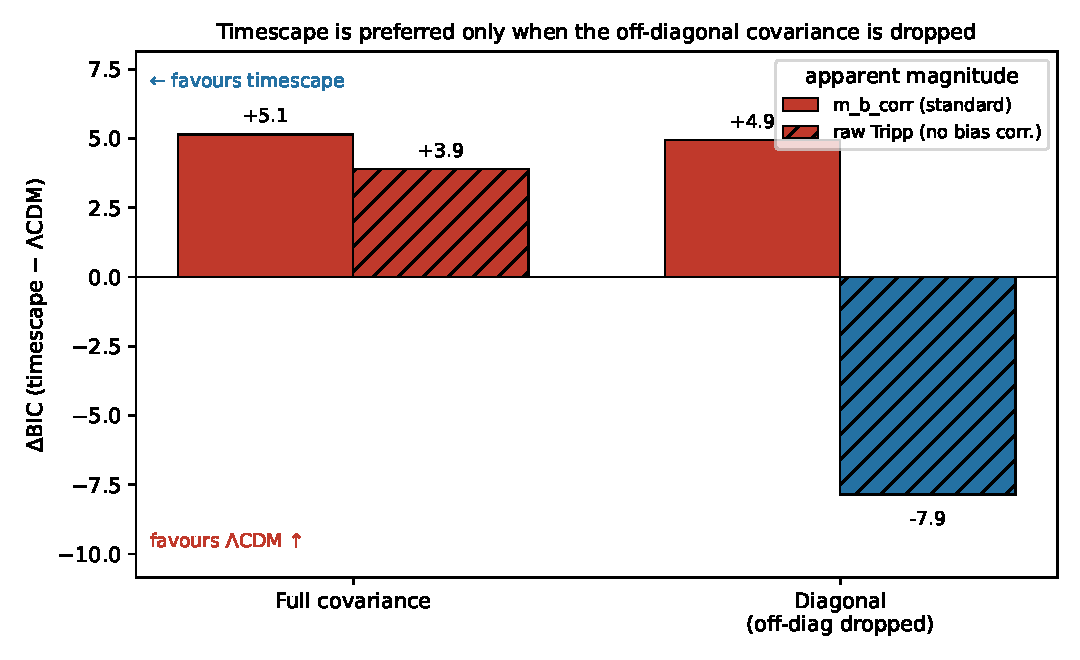
\includegraphics[width=\columnwidth]{fig_dbic}
\caption{Model-comparison verdict on Pantheon$+$ across magnitude (solid
$=m_{B,\rm corr}$, hatched $=$ raw Tripp) and covariance (full vs diagonal).
Red favours $\Lcdm$, blue favours timescape. Only the raw-Tripp$+$diagonal case
favours timescape; the full covariance favours $\Lcdm$ for every magnitude
definition.}
\label{fig:dbic}
\end{figure}

\begin{figure}[t]
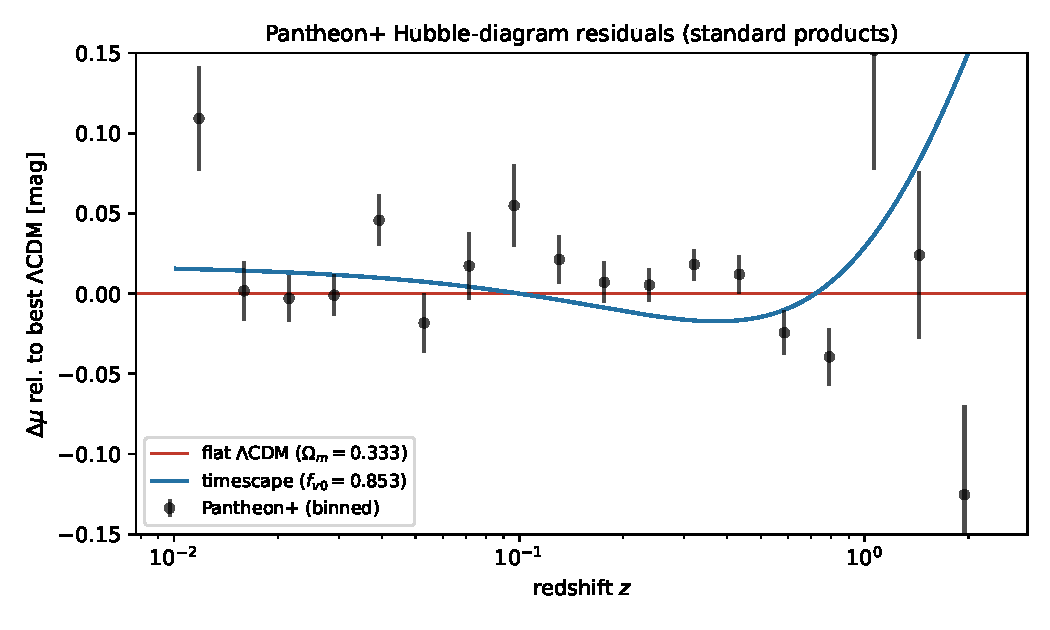
\includegraphics[width=\columnwidth]{fig_hubble}
\caption{Pantheon$+$ Hubble-diagram residuals relative to the best-fit flat
$\Lcdm$ (standard products). The best-fit timescape relation (blue) departs from
$\Lcdm$ by $<0.05$ mag over the full range, explaining the covariance
sensitivity.}
\label{fig:hubble}
\end{figure}

\subsection{Reproducing the cosmology-independent covariance}
\label{sec:seifert}
Our diagonal cases \emph{discard} the off-diagonal covariance; they are not
equivalent to the cosmology-independent covariance of \cite{Lane2025,Seifert2024},
which \emph{rebuilds} the off-diagonal (FLRW-geometry- and
peculiar-velocity-independent) terms. That covariance, with its $P{+}1690$ input
vector, is now public,\footnote{Covariance and input: Zenodo
doi:10.5281/zenodo.12729746; pipeline and construction:
\url{https://github.com/antosft/SNe-PantheonPlus-Analysis}.} so we run our
timescape-versus-$\Lcdm$ comparison directly under it, using the authors'
Nielsen--Guffanti--Sarkar hierarchical likelihood (latent SALT2 population with
profiled $\alpha,\beta$ and intrinsic dispersion, marginalised absolute
magnitude) with our own distance code, which we verify is numerically identical
to theirs; the likelihood itself we cross-check against an independent
implementation to $10^{-13}$.

\begin{table}[t]
\caption{Timescape versus flat $\Lcdm$ under the cosmology-independent
Seifert--Lane $P{+}1690$ covariance, as a function of the CMB-frame redshift cut
$z_{\min}$ (frequentist profile likelihood; $\dBIC=\mathrm{BIC}_{\rm TS}-
\mathrm{BIC}_{\Lcdm}$ with $k=9$ each, so $\dBIC=\Delta\chi^2$; both statistics
$<0$ favour timescape, $>0$ favour $\Lcdm$). $\ln B$ profiles the nuisances and
integrates the cosmological parameter (its $2\times2$-prior spread is $\pm0.3$).
The maximum-likelihood $\fvo,\Omega_{m0}$ reproduce the published values of
\cite{Lane2025}.}
\label{tab:seifert}
\begin{ruledtabular}
\begin{tabular}{lccccc}
$z_{\min}$ & $N$ & $\fvo$ & $\Omega_{m0}$ & $\dBIC$ & $\ln B$ \\
\colrule
$0.010$ & $1578$ & $0.670$ & $0.451$ & $-0.5$ & $-0.8$ \\
$0.033$ & $1169$ & $0.675$ & $0.433$ & $+1.5$ & $+0.3$ \\
$0.055$ & $1032$ & $0.680$ & $0.415$ & $+4.9$ & $+2.0$ \\
\end{tabular}
\end{ruledtabular}
\end{table}

Our frequentist maximum-likelihood fit reproduces the published values,
$\fvo=0.675$ and $\Omega_{m0}=0.433$ \cite{Lane2025}, and recovers the reported
dependence on the redshift cut (Table~\ref{tab:seifert}): timescape is marginally
favoured below the statistical-homogeneity scale ($\dBIC=-0.5$ at $z_{\min}=0.01$,
with $\ln B$ likewise mildly favouring timescape), there is no significant
preference at $z_{\min}=0.033$, and $\Lcdm$ is favoured at $z_{\min}=0.055$
($\dBIC=+4.9$). This \emph{reproduces} the qualitative finding of
\cite{Lane2025,Seifert2024}---a timescape preference concentrated below the
homogeneity scale that weakens and reverses above it---rather than refuting it.

Three caveats bound the interpretation. (i) Our frequentist $\fvo\approx0.68$ at
$z\geq0.055$ sits $\approx2\sigma$ below the $\fvo=0.737\pm0.029$ that
\cite{Seifert2024} obtain by Bayesian nested sampling; this is an
estimator difference (frequentist maximum likelihood versus Bayesian posterior on
a skewed profile), not a discrepancy---our value matches the frequentist
maximum-likelihood estimate of \cite{Lane2025}. (ii) Their headline $\ln B>5$ is
a fully-marginalised evidence for the whole sample ($z_{\min}\!\to\!0$); our
$\ln B$ profiles the nuisance parameters and integrates the single cosmological
parameter by quadrature (Occam factors assumed to cancel by the identical
nuisance structure across models), so we take $\dBIC$ as the primary statistic and
$\ln B$ as a consistency check. (iii) The $\Lcdm$ preference at $z\geq0.055$ is
mild-to-moderate ($|\dBIC|<6$), not decisive. The picture is thus sharpened rather
than overturned: under the cosmology-independent covariance the supernova
preference is a low-redshift, scale-dependent effect, not a robust whole-sample
preference for either model.

\section{Joint calibration: BAO and the CMB acoustic scale}
\label{sec:baocmb}
To test whether the dressed $\Ho\approx61\kmsmpc$ is consistent with the inverse
distance ladder, we calibrate timescape against the DESI DR2 BAO distances
\cite{DESIDR2} and the Planck acoustic scale $100\theta_*=1.04109$
\cite{Planck2018}, using the drag-epoch sound horizon $r_d$ as the standard
ruler. We compute the dressed transverse comoving distance $D_M(z)$, Hubble
distance $D_H(z)=c/H(z)$, and $D_V(z)$ from the tracker solution and fit
$(\fvo,\,\alpha\equiv c/(\Hbaro r_d))$. Since $r_d$ enters only the amplitude
$\alpha$, the redshift \emph{shape}---and hence $\fvo$---is independent of the
sound-horizon calibration.

The fit prefers $\fvo=0.636\pm0.006$ and, with the standard $r_d=147.1$~Mpc, a
dressed $\Ho=62.6\kmsmpc$: close to the dressed value of
Sec.~\ref{sec:consistency}, and recovering the independent CMB determination
$\fvo=0.627$ of \cite{Nazer2015}, which validates the calculation. However the
fit is poor, $\chi^2/\mathrm{dof}=6.7$, versus $0.89$ for flat $\Lcdm$
($\Omega_{m0}=0.30$, $\Ho=69\kmsmpc$ on the same data and pipeline); BAO alone
prefer $\fvo=0.68$. The BAO$+$CMB and supernova data prefer different void
fractions (Fig.~\ref{fig:fvtension}), which we quantify by a profile-likelihood
parameter-shift in $\fvo$: the rise in the jointly-minimised $\chi^2$ above the
sum of the separate minima, distributed as $\chi^2$ with one degree of freedom.
Against the paper's own Pantheon$+$ fit this shift is $6.6\sigma$ for the
BAO$+$CMB pairing and $4.8\sigma$ for the CMB- and $r_d$-free BAO-only pairing
($6.5\sigma$ and $4.4\sigma$ on DR1). A ladder over five supernova
standardisations and four BAO treatments puts a $3.1\sigma$ floor on the split
(from the DR1 ladder; DR2 only raises it) and
shows that it falls to $\sim1$--$2\sigma$ only when the paper's own SN fit is
replaced by the external cosmology-independent anchor $\fvo=0.737$ \emph{and} the
$\sim\!13\%$ CMB $\fvo$ systematic \cite{Nazer2015} is grafted onto the geometric
BAO-shape fit---a systematic that the $r_d$-independent BAO-only fit does not
carry. A parametric bootstrap sharpens the exclusion: of 4000 mocks drawn from a
single-void-fraction timescape truth, none reproduces the observed
SN-versus-BAO $\fvo$ split (largest $0.12$ versus the observed $0.21$), a
distribution-free exclusion of $\gtrsim3.2\sigma$.\footnote{A
Gaussian/generalised-Pareto tail extrapolation beyond the mock support gives
$\approx7.5\sigma$; we quote the distribution-free floor.} The BAO$+$CMB-alone
model comparison gives $\dBIC(\mathrm{TS}-\Lcdm)=+69.3$ ($+23.3$ on DR1). We
therefore report a robust tension between the SN- and BAO$+$CMB-preferred void
fractions---largely $r_d$-independent (it concerns the distance--redshift shape),
to be settled definitively only with a self-consistent timescape sound horizon;
the timescape literature reports concordance across these probes
\cite{Leith2008,Nazer2015}. The CMB here enters only through the acoustic-scale
point $D_M(z_*)/r_d$, not the full power spectrum; a self-consistent timescape
$r_d$ would shift $\Ho$ but not the shape-driven $\fvo$ tension, which the
BAO-only fit confirms. These figures use DESI DR2; DR1 is the more conservative
choice on every axis and we retain it as a sensitivity check.

\begin{figure}[t]
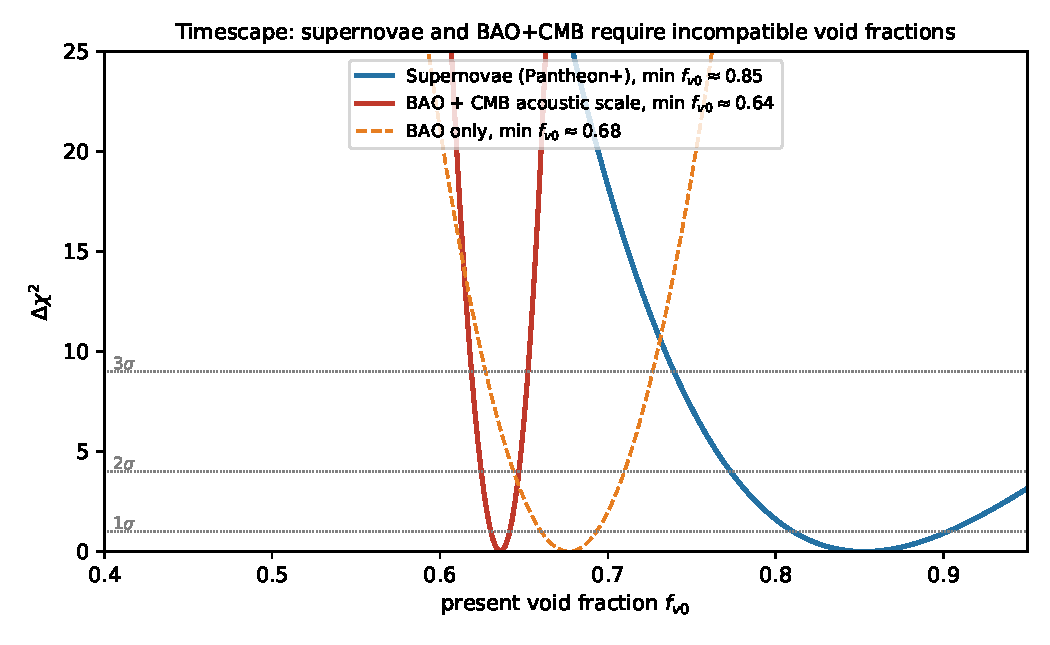
\includegraphics[width=\columnwidth]{fig_fvtension}
\caption{$\Delta\chi^2$ for the present void fraction $\fvo$ from supernovae
(blue), BAO$+$CMB (red), and BAO alone (orange). The supernova and BAO$+$CMB
minima are separated by $\Delta\fvo\approx0.2$ with non-overlapping confidence
regions: no single timescape model fits both.}
\label{fig:fvtension}
\end{figure}

\subsection{Acceleration, and an evolving-dark-energy comparison}
\label{sec:w0wa}
Apparent acceleration is present in every best fit, so the comparison is not an
artifact of one model lacking it: the dressed timescape deceleration parameter is
$q_0=-0.02$ to $-0.04$ (a weak apparent effect from the lapse, with the bare
$\bar q_0>0$), versus $q_0=-0.54$ for $\Lcdm$ (joint fit). As a motivated alternative that
instead \emph{modifies} the acceleration history, we also fit the CPL
evolving-dark-energy model $w(a)=w_0+w_a(1-a)$ jointly to SN$+$BAO$+$CMB. It
returns $w_0=-0.87$, $w_a=-0.48$---the thawing direction hinted at by DESI
\cite{DESI2024}---with $q_0=-0.40$, but improves the fit by only
$\Delta\chi^2=3.9$ for two extra parameters ($\dBIC=+10.8$ versus $\Lcdm$), so it
is not significantly preferred. Table~\ref{tab:joint} collects the joint fits:
$\Lcdm$ is the most economical, evolving dark energy a mild non-significant
improvement in the DESI direction, and timescape strongly disfavoured
($\dBIC=+67$) because no single void fraction fits SN and BAO$+$CMB.

\begin{table}[t]
\caption{Joint SN$+$BAO$+$CMB fits ($N=1593$), identical harness. $\dBIC$
relative to $\Lcdm$; $q_0<0$ denotes acceleration. BAO data here are DESI DR1;
the DR2 recalibration of Sec.~\ref{sec:baocmb} only sharpens the timescape
disfavour.}
\label{tab:joint}
\begin{ruledtabular}
\begin{tabular}{lcccc}
Model & parameters & $\Ho$ & $q_0$ & $\dBIC$\\
\colrule
$\Lcdm$ & $\Omega_{m0}=0.305$ & $68.6$ & $-0.54$ & $0$\\
$w_0w_a$CDM & $\Omega_{m0}=0.31,w_0=-0.87,w_a=-0.48$ & $68.0$ & $-0.40$ & $+10.8$\\
timescape & $\fvo=0.64$ & $63.1$ & $-0.02$ & $+67.1$\\
\end{tabular}
\end{ruledtabular}
\end{table}

\subsection{Simplifications}
\label{sec:simpl}
The calibration makes explicit approximations, none of which affect the central
SN--BAO$+$CMB incompatibility (which is geometric and, in the BAO-only form,
independent of $r_d$ and the CMB): (i) the CMB enters only through the
acoustic-scale point $D_M(z_*)/r_d$, not the full power spectrum or the
$(R,\ell_A,\omega_b)$ compression; (ii) we adopt the standard early-physics
$r_d=147.1$~Mpc rather than a self-consistent timescape sound horizon, which
would rescale $\Ho$ but not the shape-driven $\fvo$; (iii) the timescape tracker
is the late-time attractor (reached by $z\sim37$), so $D_M(z_*)$ uses it slightly
beyond its regime, though the comoving distance is dominated by $z\lesssim$ few;
(iv) radiation is neglected in the late-time distance integrals; (v) $\Lcdm$ is
taken spatially flat.

\section{The wider void and backreaction family}
\label{sec:voids}
To test whether the timescape result is special, we applied the identical
SN$+$BAO$+$CMB harness to the principal dark-energy-free inhomogeneous
cosmologies (Table~\ref{tab:voids}). Each distance--redshift relation was
implemented from primary sources and validated against published or analytic
limits; the SN absolute-magnitude offset and the BAO ruler $c/(\Ho r_d)$ were
marginalised as before.

The outcome is uniform. (i) The LTB giant-void model (constrained GBH
\cite{GBH2008}) reproduces SN acceleration with a deep central void but, like
timescape, prefers a \emph{deeper} void for SNe than for BAO$+$CMB (joint
$\dBIC\approx+717$); its central $\Ho$ reaches only $\sim\!55$--$59$, and it is
independently excluded by the kinetic Sunyaev--Zel'dovich effect
\cite{ZhangStebbins2011,Camarena2022}. (ii) The R\"as\"anen peak/backreaction model
\cite{Rasanen2008,Rasanen2009} is parameter-free and, by its authors' own
evaluation, does not even produce acceleration ($\bar q>0$,
$|\Omega_{\mathcal Q}|<0.04$); promoting the backreaction to a free parameter, SNe
demand values beyond its physical reach and the joint fit gives
$\dBIC\approx+72$ (above timescape's $+67$ once its extra backreaction parameter
is charged the Occam penalty the same harness applies to $w_0w_a$CDM and LTB). (iii) The Buchert backreaction ``morphon'' template
\cite{Larena2009} fits SNe but fails BAO$+$CMB catastrophically
($\dBIC\sim+1.6\times10^3$). (iv) The Szekeres model \cite{MeuresBruni2011} has no
closed-form isotropic distance and could not be reliably fit here; the literature
verdict (kSZ-capped void depth, residual $\sim\!3\sigma$ tension
\cite{Camarena2022}) is that it does not resolve the tension. (v) The local KBC
void \cite{KBC2013,Haslbauer2020}---which \emph{retains} dark energy---leaves
BAO$+$CMB untouched and earns no statistical preference (a fixed literature-depth
void worsens the joint fit by $\dBIC\approx+165$, growing monotonically with
depth, so the no-void $\Lcdm$ limit is preferred); a void deep enough to reach
$73$ is both deeper than observed
and disfavoured by the supernova Hubble-flow shape
\cite{Kenworthy2019,Camarena2022}.

Every dark-energy-free void/backreaction model thus shows the same
SN-versus-BAO$+$CMB parameter split as timescape, and none reaches the local
$\Ho$: the failure is generic to the class, not specific to one model. The
$\dBIC$ magnitudes from this geometric harness are approximate (single CMB
acoustic point, standard $r_d$), but the qualitative verdict is robust and, for
the LTB/Szekeres subclass, reinforced by the independent kSZ exclusion.

\begin{table}[t]
\caption{Uniform SN$+$BAO$+$CMB test of void/backreaction cosmologies on the same
harness. ``DE-free'' marks models that eliminate dark energy. $\dBIC$ is relative
to $\Lcdm$ (joint $\chi^2=1402$); larger is more disfavoured. None resolves the
tension.}
\label{tab:voids}
\begin{ruledtabular}
\begin{tabular}{lccl}
Model & DE-free & joint $\dBIC$ & verdict \\
\colrule
$\Lcdm$ (ref.)   & no  & $0$              & --- \\
$w_0w_a$CDM      & no  & $+11$            & no (mild DESI-direction hint) \\
Timescape        & yes & $\sim\!+67$      & no \\
LTB void (GBH)   & yes & $\sim\!+717$     & no ($+$kSZ-excluded) \\
R\"as\"anen peak & yes & $\sim\!+72$      & no (predicts no acceleration) \\
Buchert morphon  & yes & $\sim\!+1600$    & no \\
Szekeres         & yes & intractable      & no (literature $+$ kSZ) \\
KBC local void   & no  & $0$ (no-void lim.) & no (needs unobserved deep void) \\
\end{tabular}
\end{ruledtabular}
\end{table}

\section{Prior dark-energy-free resolutions and their status}
\label{sec:related}
The proposal that apparent acceleration---and, by extension, the Hubble
tension---reflects the inhomogeneity of the late Universe rather than a new
energy component has a long lineage, and our same-footing test sits within a
literature of single-model studies. We summarise that landscape here, separating
the proponents' claims from the principal critiques, so that our uniform survey
(Sec.~\ref{sec:voids}) and the void-family Table~\ref{tab:voids} can be read in
context.

\emph{The timescape program.} Timescape grew out of Wiltshire's resolution of
the cosmological averaging problem \cite{Wiltshire2007,Wiltshire2009}, built on
the Buchert spatial-averaging formalism \cite{Buchert2000}, with the bare/dressed
distinction as its conceptual core: a wall observer fitting FLRW infers
parameters that differ from the volume average. Leith, Ng \& Wiltshire
\cite{Leith2008} reported the first multi-probe concordance fit (SNe$+$CMB$+$BBN
mutually consistent without dark energy at a low dressed $\Ho$), Duley, Nazer \&
Wiltshire \cite{Duley2013} added a radiation fluid to reach recombination, and
Nazer \& Wiltshire \cite{Nazer2015} fitted the CMB acoustic peaks, quoting a
dressed $\Ho\simeq61\kmsmpc$ with large ($\sim8$--$13\%$) systematics. On
supernovae the verdict has been sensitive throughout: Smale \& Wiltshire
\cite{Smale2011} found timescape preferred for MLCS2k2-reduced samples but
disfavoured for SALT-reduced ones, identifying the light-curve fitter as the
dominant systematic, and Dam, Heinesen \& Wiltshire \cite{Dam2017} found
timescape statistically indistinguishable from flat $\Lcdm$ on JLA with marginal
apparent acceleration. The review of Wiltshire \cite{Wiltshire2014} frames dark
energy as a coarse-graining artifact and rests part of the case on a sub-$100\,
h^{-1}$Mpc Hubble-flow variance and a claimed Local-Group-frame uniformity
\cite{Wiltshire2013}---a cosmic-rest-frame inference that remains contested. The
recent revival sharpens the supernova claim: Lane et al.\ \cite{Lane2025} and
Seifert et al.\ \cite{Seifert2024} reanalyse Pantheon$+$ with a covariance
constructed to be independent of FLRW geometry and peculiar-velocity corrections
and report very strong Bayesian evidence ($\ln B>5$) for timescape over $\Lcdm$,
with the preference persisting beyond the statistical-homogeneity scale. We
test these claims directly (Sec.~\ref{sec:seifert}): running our comparison under
their now-public cosmology-independent covariance, we reproduce their published
maximum-likelihood void fraction ($\fvo=0.675$) and their reported redshift-cut
dependence---timescape marginally favoured below the statistical-homogeneity scale
and $\Lcdm$ above it. The supernova preference is thus real but scale-dependent, a
low-redshift effect rather than a robust whole-sample result, and its Bayesian
magnitude ($\ln B>5$) reflects their fully-marginalised evidence for the whole
sample where ours is a nuisance-profiled approximation.

\emph{Backreaction and giant voids.} A parallel tradition seeks acceleration
directly from spatial averaging: R\"as\"anen's mechanism \cite{Rasanen2006}, in
which faster-expanding voids coming to dominate the volume drive an effective
acceleration, which his own quantitative peak-model evaluation
\cite{Rasanen2008} then found too weak, and the Buchert ``morphon'' repackaging
of backreaction as an effective scalar \cite{Larena2009}. Whether backreaction
can be dynamically significant is the subject of a long, still-open exchange:
Green \& Wald argue the metric is everywhere close to FLRW so backreaction is
trace-free and cannot source acceleration \cite{GreenWald2014}, while an
eleven-author rebuttal contends their scheme misses the non-local averaging
effects that matter \cite{Buchert2015}; recent first-principles GR computations
on the real local Universe find the kinematical backreaction small ($\lesssim
1\%$) even as the integrated spatial curvature reaches $\sim10\%$
\cite{Galoppo2026}, and full numerical-relativity void statistics supply a
$10$--$30\%$ void-overexpansion that motivates the void-fraction parameter
\cite{Williams2024}. The LTB/Szekeres giant-void line \cite{GBH2008} fits SNe
with a deep central void but is bounded sharply from outside: radial BAO and a
low-$\Ho$/fine-tuning dilemma \cite{ZibinMossScott}, a multi-probe exclusion
\cite{MossZibinScott2011}, and---decisively---the kinetic Sunyaev--Zel'dovich
effect, an unavoidable consequence of large radial inhomogeneity that rules out
adiabatic Gpc voids \cite{ZhangStebbins2011}. The distinct \emph{local}-void
($\Ho$-outflow) idea, including the deep KBC void \cite{KBC2013,Haslbauer2020},
is separately disfavoured: the local Hubble-flow shape shows no outflow of the
required size \cite{Kenworthy2019} and the supposed void resolution is an artifact
of the redshift range used to calibrate $\Ho$ \cite{Camarena2022}.

\emph{The recent (2023--26) context.} Several developments have renewed interest.
The DESI inverse-distance-ladder gives $\Ho\simeq68\kmsmpc$ and hints at evolving
dark energy ($w_0>-1$, $w_a<0$) \cite{DESI2024}, which the no-dark-energy programs
read as room for an inhomogeneity-driven effective equation of state. The
tension's apparent magnitude has also softened on the calibrator axis: the
TRGB ladder of the Chicago--Carnegie Hubble Program gives $\Ho\simeq68$--$70$,
only $\sim1$--$1.5\sigma$ from Planck \cite{Freedman2024,CCHP2025}, so the
$5\sigma$ figure is largely SH0ES-Cepheid-specific. Against this, the
review/ranking literature has consistently placed the inhomogeneity class below
early-time new physics: the field's solution catalogues assign it a weaker
verdict \cite{DiValentino2021}, and metric-based rankings find late-Universe and
local mechanisms cannot resolve $\Ho$ under joint BAO$+$SN constraints
\cite{Schoneberg2022}.

\emph{This work in context.} The studies above are overwhelmingly single-model:
each proponent paper fits one framework, and each critique bounds one mechanism.
Our contribution is a \emph{uniform} test---the identical SN$+$BAO$+$CMB harness,
with the same likelihood, marginalisation, and model-comparison statistic applied
across the whole dark-energy-free family (Sec.~\ref{sec:voids})---which makes the
recurring SN-versus-BAO$+$CMB parameter split visible as a property of the class
rather than of any one model. It complements, rather than supersedes, the
detailed single-model analyses: where the proponents retain a
cosmology-independent supernova covariance whose recent public release now makes
reproduction possible, and where the critiques deploy probes (kSZ, radial BAO)
outside our distance-only harness, our test adds the same-footing comparison that
the existing literature lacks.

\section{Discussion}
\label{sec:discussion}
Three conclusions follow. First, interpreted within timescape the early- and
late-Universe \emph{dressed} $\Ho$ agree at $\approx61$, and the local excess is
of the predicted magnitude (a fresh SH0ES-calibrator-anchored late-time fit
returns $73.0\pm1.0$, the locally-biased value the model predicts, not $61$); but
this is a recasting, not a reconciliation near $70$, and the global value lies
below Planck. Second, the supernova
model-comparison verdict is contingent on the covariance treatment: it favours
$\Lcdm$ under the full public covariance and timescape only when the off-diagonal
terms are removed. Third, when timescape is required to fit supernovae, BAO, and
the CMB acoustic scale \emph{together}, the SN- and BAO$+$CMB-preferred void
fractions differ ($\Delta\fvo\approx0.1$--$0.2$) and timescape fits the BAO$+$CMB
geometry worse than $\Lcdm$; the split is a robust profile-likelihood parameter
shift (up to $6.6\sigma$, $4.8\sigma$ in the CMB- and $r_d$-free pairing,
$\gtrsim3.2\sigma$ by parametric bootstrap), softening to $\sim1$--$2\sigma$ only
under the external cosmology-independent anchor combined with the CMB $\fvo$
systematic (Sec.~\ref{sec:baocmb}). The early/late dressed-$\Ho$ consistency of Sec.~\ref{sec:consistency}
is thus genuine, but whether one parameter set also describes the combined
distance data is unsettled on present evidence, pending the self-consistent sound
horizon and cosmology-independent covariance. Notably the same SN-versus-BAO$+$CMB
split recurs across the whole void/backreaction family (Sec.~\ref{sec:voids}),
suggesting it is generic to dark-energy-free inhomogeneous models rather than
specific to timescape.

These results sit within known open problems: the timescape CMB fit
\cite{Nazer2015} matches the acoustic-peak structure by adapting an $\Lcdm$
template rather than from first principles; BAO and growth constraints are far
less developed than for $\Lcdm$; and whether backreaction can be dynamically
significant is disputed \cite{GreenWald2014,Buchert2015}.

\subsection{Is the split directional averaging, or model rigidity? A line-of-sight test}
\label{sec:losvoids}
Timescape applies one averaged distance--redshift curve to every sightline, yet the local
void content is \emph{measured} at low redshift. We tested directly whether injecting it changes
the supernova verdict, using the reconstructed 2M$++$ galaxy density field
\cite{Carrick2015} along the line of sight to each of the 573 Pantheon$+$ supernovae
($460$ distinct) inside the reconstruction's reliable radius ($\lesssim200\,h^{-1}$Mpc,
$z\lesssim0.067$); redshifts are placed with $z_{\rm CMB}$, not the peculiar-velocity-corrected
$z_{\rm HD}$, to avoid regressing the data on the same 2M$++$ field.

Three findings, each a null for the ``directional-averaging'' hypothesis. First, a generalised-least-squares
regression of the Hubble residuals on the per-sightline void fraction, under the full
covariance, is consistent with zero once calibrated against a sky-rotation null
($-0.9\sigma$); the naive regression error understates the scatter by $\approx2.7\times$
because it ignores the covariate's spatial coherence and the covariance's coherent modes, so an
apparent $\sim\!2\sigma$ signal is sub-threshold and does not survive. Second, a one-parameter
per-sightline extension of the tracker (an expansion-variance coupling to the measured void excess)
improves the fit by only $\Delta\chi^{2}\approx0.6$ and leaves $\hat\fvo$ at $0.85$: random
rotations of the field help the fit as much on average (rotation-null $p\approx0.6$). Third, the
maximal per-sightline magnitude modulation allowed by the data is $\lesssim0.05$\,mag, a few percent
of the per-supernova error and steeply weighted to $z\lesssim0.1$, because $\mathrm{Var}(F)\sim
L_{\rm void}/D(z)$ shrinks along longer beams. Measured structure therefore adds no information
at Pantheon$+$ precision: the single-parameter \emph{average} is not the bottleneck, and the
low-redshift origin of the supernova preference is a variance/covariance effect rather than a
cosmological signal.

Two further checks locate the tension. Externally, the supernova-preferred $\fvo\approx0.85$
exceeds the observed present-day void volume fraction under any structure-based definition
(numerical-relativity watershed void statistics bracket $\approx0.50$--$0.62$
\cite{Williams2024}), whereas $\fvo\approx0.64$ coincides with both that bracket and
timescape's own Planck fits \cite{Nazer2015}. And a free, spline-parametrised smooth expansion
history fit jointly to supernovae, BAO, and the CMB acoustic scale matches $\Lcdm$
($\Delta\chi^{2}=10$ for five extra parameters, $p=0.07$) and sits far below the timescape
tracker ($\Delta\chi^{2}\approx67$). A smooth history \emph{can} reconcile the three datasets;
the timescape tracker cannot. The SN-versus-BAO$+$CMB split is thus the rigidity of the
one-parameter averaged history---one $\fvo$ forced to serve a low-redshift supernova shape and the
BAO$+$CMB geometry at once---not a failure to resolve directional structure, and not an
irreducible supernova--BAO shape disagreement. This is a robustness result: it strengthens, rather
than overturns, the recasting interpretation of Sec.~\ref{sec:discussion}.

\section{What a decisive test requires}
\label{sec:future}
(i) The cosmology-independent, FLRW-geometry- and peculiar-velocity-independent
Pantheon$+$ covariance of Seifert et al.\ is now public and we have run it under
our harness (Sec.~\ref{sec:seifert}): the supernova preference is
scale-dependent---marginally timescape below the statistical-homogeneity scale
($\dBIC=-0.5$), $\Lcdm$ above ($\dBIC=+4.9$ at $z\geq0.055$)---reproducing the
proponents' redshift-cut trend and their maximum-likelihood void fraction. A
fully-marginalised Bayesian evidence, versus our nuisance-profiled approximation,
would sharpen the low-$z$ magnitude but not the sign; that is what remains.
(ii) A joint re-fit of Pantheon$+$ and Planck within timescape with the dressed
$\Ho$ \emph{free}, and a self-consistent timescape sound-horizon/BAO calibration,
so early and late $\Ho$ are genuine independent measurements; the
calibrator-anchored late-time half of this test is carried out in
Sec.~\ref{sec:consistency}, leaving the self-consistent sound horizon. (iii) A direct
measurement of the radial profile of the apparent $\Ho$ versus scale, to test the
predicted expansion variance that the local-excess cross-check assumes.

\section{Conclusions}
\label{sec:concl}
Within timescape the early- and late-Universe dressed Hubble constants agree to
$\lesssim0.5\sigma$ (versus $\approx4.9\sigma$ in $\Lcdm$), and the local excess
matches the predicted void-scale variance---but the model recasts rather than
reconciles the tension, collapsing both canonical values to $\approx61\kmsmpc$,
below Planck. Our independent Pantheon$+$ reanalysis finds $\Lcdm$ favoured under our own
full-covariance reductions ($\dBIC=+3.9$ to $+5.1$; exact $\ln B=+1.3$ to $+1.8$),
with a timescape preference appearing when the off-diagonal covariance is discarded
(stat-only $\ln B=5.4$--$5.9$ for timescape). Run under the proponents' now-public
cosmology-independent covariance, our fit reproduces their published
maximum-likelihood values and their scale-dependent result: timescape marginally
favoured below the statistical-homogeneity scale ($\dBIC=-0.5$ at $z>0.01$),
$\Lcdm$ above it ($\dBIC=+4.9$ at $z\geq0.055$). The supernova preference is thus
real but a low-redshift, scale-dependent effect, not a robust whole-sample
preference. A joint calibration against DESI DR2 BAO and the Planck
acoustic scale fits worse than $\Lcdm$ ($\chi^2/\mathrm{dof}=6.7$ vs $0.89$) and
prefers a void fraction ($\fvo\simeq0.64$) in tension with the supernova value
($0.74$--$0.85$) at $4.8$--$6.6\sigma$ (profile parameter-shift;
$\gtrsim3.2\sigma$ by parametric bootstrap), softening to $\sim1$--$2\sigma$ only
under the external cosmology-independent anchor plus the CMB $\fvo$ systematic. The dressed-$\Ho$
numbers \emph{are} reconciled within timescape ($\approx61\kmsmpc$); what remains
open is whether one parameter set also fits the combined SN$+$BAO$+$CMB distances.
A uniform test of the wider void/backreaction family (Sec.~\ref{sec:voids}) finds
the same SN-vs-BAO$+$CMB split in every dark-energy-free model and none reaching
the local $\Ho$, with the LTB subclass independently excluded by the kSZ effect.
Finally, the tension's magnitude is calibrator-dependent: the TRGB ladder gives
$\Ho\simeq68$--$70$, $\sim1$--$1.5\sigma$ from Planck, so the $5\sigma$ tension is
largely an artifact of the SH0ES Cepheid calibration. On present public data,
eliminating dark energy via inhomogeneity does not resolve the Hubble tension.

\begin{acknowledgments}
The author used the Claude large language model (Anthropic) as a
research-assistance tool: for primary-literature retrieval, for implementing and
running the supernova analysis of Sec.~\ref{sec:sne}, and for drafting. All
sources, equations, code, and numerical results were verified by the author, who
takes full responsibility for the content and any errors. This work received no
funding.
\end{acknowledgments}

\section*{Data and code availability}
\label{sec:avail}
This work uses the public Pantheon$+$ release \cite{Scolnic2022,Brout2022}
(\url{https://github.com/PantheonPlusSH0ES/DataRelease}). The analysis code
(timescape and $\Lcdm$ distance modules, the magnitude$\times$covariance
decomposition, the validation tests, and the figure scripts) is available from
the author and will be deposited publicly on publication.

\begin{thebibliography}{99}
\bibitem{Riess2022} A.~G.~Riess \emph{et al.}, Astrophys.\ J.\ Lett.\ \textbf{934}, L7 (2022), arXiv:2112.04510.
\bibitem{Planck2018} Planck Collaboration, Astron.\ Astrophys.\ \textbf{641}, A6 (2020), arXiv:1807.06209.
\bibitem{Riess2024JWST} A.~G.~Riess \emph{et al.}, Astrophys.\ J.\ Lett.\ \textbf{962}, L17 (2024), arXiv:2401.04773.
\bibitem{Freedman2024} W.~L.~Freedman \emph{et al.} (2024), arXiv:2408.06153.
\bibitem{DESI2024} DESI Collaboration (2024), arXiv:2404.03002.
\bibitem{DESIDR2} DESI Collaboration, ``DESI DR2 Results II: Measurements of Baryon Acoustic Oscillations and Cosmological Constraints'' (2025), arXiv:2503.14738.
\bibitem{Wiltshire2007} D.~L.~Wiltshire, Phys.\ Rev.\ Lett.\ \textbf{99}, 251101 (2007), arXiv:0709.0732.
\bibitem{Wiltshire2009} D.~L.~Wiltshire, Phys.\ Rev.\ D \textbf{80}, 123512 (2009), arXiv:0909.0749.
\bibitem{Buchert2000} T.~Buchert, Gen.\ Relativ.\ Gravit.\ \textbf{32}, 105 (2000), arXiv:gr-qc/9906015.
\bibitem{Leith2008} B.~M.~Leith, S.~C.~C.~Ng, D.~L.~Wiltshire, Astrophys.\ J.\ Lett.\ \textbf{672}, L91 (2008), arXiv:0709.2535.
\bibitem{Duley2013} J.~A.~G.~Duley, M.~A.~Nazer, D.~L.~Wiltshire, Class.\ Quantum Grav.\ \textbf{30}, 175006 (2013), arXiv:1306.3208.
\bibitem{Nazer2015} M.~A.~Nazer, D.~L.~Wiltshire, Phys.\ Rev.\ D \textbf{91}, 063519 (2015), arXiv:1410.3470.
\bibitem{Smale2011} P.~R.~Smale, D.~L.~Wiltshire, Mon.\ Not.\ R.\ Astron.\ Soc.\ \textbf{413}, 367 (2011), arXiv:1009.5855.
\bibitem{Wiltshire2013} D.~L.~Wiltshire, P.~R.~Smale, T.~Mattsson, R.~Watkins, Phys.\ Rev.\ D \textbf{88}, 083529 (2013), arXiv:1201.5371.
\bibitem{Dam2017} L.~H.~Dam, A.~Heinesen, D.~L.~Wiltshire, Mon.\ Not.\ R.\ Astron.\ Soc.\ \textbf{472}, 835 (2017), arXiv:1706.07236.
\bibitem{Lane2025} Z.~G.~Lane, A.~Seifert, R.~Ridden-Harper, D.~L.~Wiltshire, Mon.\ Not.\ R.\ Astron.\ Soc.\ \textbf{536}, 1752 (2025), arXiv:2311.01438.
\bibitem{Seifert2024} A.~Seifert, Z.~G.~Lane, M.~Galoppo, R.~Ridden-Harper, D.~L.~Wiltshire, Mon.\ Not.\ R.\ Astron.\ Soc.\ Lett.\ \textbf{537}, L55 (2025), arXiv:2412.15143.
\bibitem{Scolnic2022} D.~Scolnic \emph{et al.}, Astrophys.\ J.\ \textbf{938}, 113 (2022), arXiv:2112.03863.
\bibitem{Brout2022} D.~Brout \emph{et al.}, Astrophys.\ J.\ \textbf{938}, 110 (2022), arXiv:2202.04077.
\bibitem{Tripp1998} R.~Tripp, Astron.\ Astrophys.\ \textbf{331}, 815 (1998).
\bibitem{KassRaftery1995} R.~E.~Kass, A.~E.~Raftery, J.\ Am.\ Stat.\ Assoc.\ \textbf{90}, 773 (1995).
\bibitem{GreenWald2014} S.~R.~Green, R.~M.~Wald, Class.\ Quantum Grav.\ \textbf{31}, 234003 (2014), arXiv:1407.8084.
\bibitem{Buchert2015} T.~Buchert \emph{et al.}, Class.\ Quantum Grav.\ \textbf{32}, 215021 (2015), arXiv:1505.07800.
\bibitem{CCHP2025} T.~J.~Hoyt, I.~S.~Jang, W.~L.~Freedman \emph{et al.}, ``The Chicago--Carnegie Hubble Program: improving the calibration of SNe~Ia with JWST measurements of the tip of the red giant branch'' (2025), arXiv:2503.11769.
\bibitem{GBH2008} J.~Garc\'ia-Bellido, T.~Haugb\o lle, J.\ Cosmol.\ Astropart.\ Phys.\ \textbf{04}, 003 (2008), arXiv:0802.1523.
\bibitem{ZibinMossScott} J.~P.~Zibin, A.~Moss, D.~Scott, Phys.\ Rev.\ Lett.\ \textbf{101}, 251303 (2008), arXiv:0809.3761.
\bibitem{Camarena2022} D.~Camarena, V.~Marra, Z.~Sakr, C.~Clarkson, Class.\ Quantum Grav.\ \textbf{39}, 184001 (2022), arXiv:2205.05422.
\bibitem{Rasanen2008} S.~R\"as\"anen, J.\ Cosmol.\ Astropart.\ Phys.\ \textbf{04}, 026 (2008), arXiv:0801.2692.
\bibitem{Rasanen2009} S.~R\"as\"anen, J.\ Cosmol.\ Astropart.\ Phys.\ \textbf{02}, 011 (2009), arXiv:0812.2872.
\bibitem{Larena2009} J.~Larena, J.-M.~Alimi, T.~Buchert, M.~Kunz, P.-S.~Corasaniti, Phys.\ Rev.\ D \textbf{79}, 083011 (2009), arXiv:0808.1161.
\bibitem{MeuresBruni2011} N.~Meures, M.~Bruni, Mon.\ Not.\ R.\ Astron.\ Soc.\ \textbf{419}, 1937 (2012), arXiv:1107.4433.
\bibitem{KBC2013} R.~C.~Keenan, A.~J.~Barger, L.~L.~Cowie, Astrophys.\ J.\ \textbf{775}, 62 (2013), arXiv:1304.2884.
\bibitem{Haslbauer2020} M.~Haslbauer, I.~Banik, P.~Kroupa, Mon.\ Not.\ R.\ Astron.\ Soc.\ \textbf{499}, 2845 (2020), arXiv:2009.11292.
\bibitem{Kenworthy2019} W.~D.~Kenworthy, D.~Scolnic, A.~Riess, Astrophys.\ J.\ \textbf{875}, 145 (2019), arXiv:1901.08681.
\bibitem{Wiltshire2014} D.~L.~Wiltshire, ``Cosmic structure, averaging and dark energy'', in \emph{Cosmology and Gravitation: XVth Brazilian School of Cosmology and Gravitation}, eds.\ M.~Novello, S.~E.~Perez Bergliaffa (Cambridge Scientific Publishers, 2014), pp.~203--244, arXiv:1311.3787.
\bibitem{Rasanen2006} S.~R\"as\"anen, J.\ Cosmol.\ Astropart.\ Phys.\ \textbf{11}, 003 (2006), arXiv:astro-ph/0607626.
\bibitem{MossZibinScott2011} A.~Moss, J.~P.~Zibin, D.~Scott, Phys.\ Rev.\ D \textbf{83}, 103515 (2011), arXiv:1007.3725.
\bibitem{ZhangStebbins2011} P.~Zhang, A.~Stebbins, Phys.\ Rev.\ Lett.\ \textbf{107}, 041301 (2011), arXiv:1009.3967.
\bibitem{DiValentino2021} E.~Di~Valentino \emph{et al.}, Class.\ Quantum Grav.\ \textbf{38}, 153001 (2021), arXiv:2103.01183.
\bibitem{Schoneberg2022} N.~Sch\"oneberg \emph{et al.}, Phys.\ Rept.\ \textbf{984}, 1 (2022), arXiv:2107.10291.
\bibitem{Williams2024} M.~J.~Williams, H.~J.~Macpherson, D.~L.~Wiltshire, C.~Stevens, Mon.\ Not.\ R.\ Astron.\ Soc.\ \textbf{536}, 2645 (2025), arXiv:2403.15134.
\bibitem{Galoppo2026} M.~Galoppo, T.~Buchert, P.~Mourier, ``Backreaction and the role of spatial curvature in the cosmic neighborhood'', Astrophys.\ J.\ Lett.\ \textbf{1002}, L39 (2026), arXiv:2605.05454.
\bibitem{Carrick2015} J.~Carrick, S.~J.~Turnbull, G.~Lavaux, M.~J.~Hudson, Mon.\ Not.\ R.\ Astron.\ Soc.\ \textbf{450}, 317 (2015), arXiv:1504.04627.
\end{thebibliography}

\end{document}
